\documentclass[11pt, a4paper]{article}
\usepackage{apacite}
\usepackage{natbib}
\usepackage[utf8x]{inputenc}
\usepackage[T1]{fontenc}
\usepackage[icelandic]{babel}
\usepackage{amsmath, amsthm, amssymb, amsfonts}
\usepackage{graphicx}
\usepackage{tikz}
\usepackage{tkz-euclide}
\usetkzobj{all}
\usepackage{listings}
\usepackage{hyperref}
\usepackage{pgfplots}
\usepackage{geometry}
\usepackage{setspace} 
\usepackage{pdflscape}
\usepackage{mathtools}
\usepackage{fixltx2e}
\usepackage{array}
\setlength\parindent{0pt}
\newtheorem*{problem}{\emph{Problem}}
\newtheorem*{solution}{\emph{Solution}}
\newcommand*\rfrac[2]{{}^{#1}\!/_{#2}} %small fraction
\begin{document}
\begin{titlepage}
\begin{center}

\textsc{\huge Haust 2016}\\[1.5cm]

\textsc{\huge Hönnun og smíði hugbúnaðar}\\[0.2cm]
\textsc{\huge T-302-THYD}\\[1.5cm]

\end{center}
{ \huge RuTube system design document\\[1.5cm] }
% Author and supervisor
\Large {
\emph{Nemandi:}\\
Steinn Elliði Pétursson\\[0.5cm]
\emph{Kennitala:}\\
250594-2759\\[0.5cm]
\emph{Nemandi:}\\
Janus Þór Kristjánsson\\[0.5cm]
\emph{Kennitala:}\\
300894-2249\\[0.5cm]
{\large \today}\\[0.5cm]
\emph{Kennari:} \\
Magnús Eðvald Björnsson}\\

\end{titlepage}
\leavevmode

\newpage
    {\LARGE \textbf{Overview}}\\~\\
    \textbf{1. Introduction}\\
    \textbf{2. Context diagram}\\
    \textbf{3. Container diagram}\\
    \textbf{4. Component diagram}\\
    \textbf{5. REST URI}\\
    \textbf{6. Database schema}\\
    
\newpage
	\section{Introduction}
		The RuTube system is a system that stores and displays channels with videos for users. Users can subscribe and interact with channels by adding and deleting their own content into the system. Following are various diagrams explaining the system with different levels of abstraction starting with the most abstract one, the context diagram. This document also contains a REST URI for external communication with the system as well as a database schema for users, videos and channels.
\newpage
	\section{Context diagram}
	This diagram shows how the RuTube system interacts with other systems and users.\\
		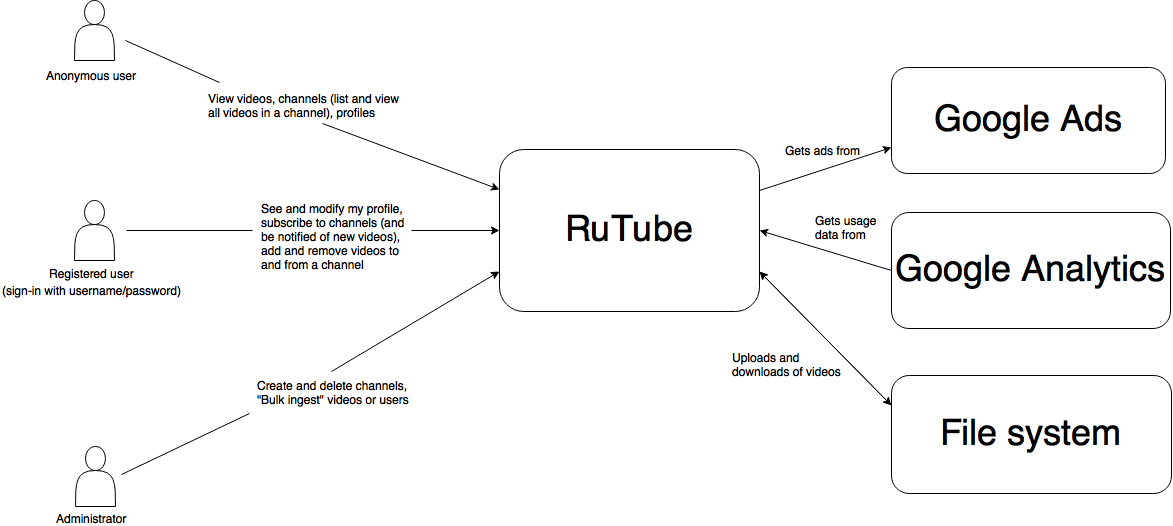
\includegraphics[height=8cm]{/Users/steinn/Documents/tolHR2016haust/T-302-HONN/Assign3honn/context_diagram.png}

\newpage
	\section{Container diagram}
		This diagram displays the system as a whole with a very high level of abstraction to help the reader get a grasp of how the different parts of the system interact.\\~\\
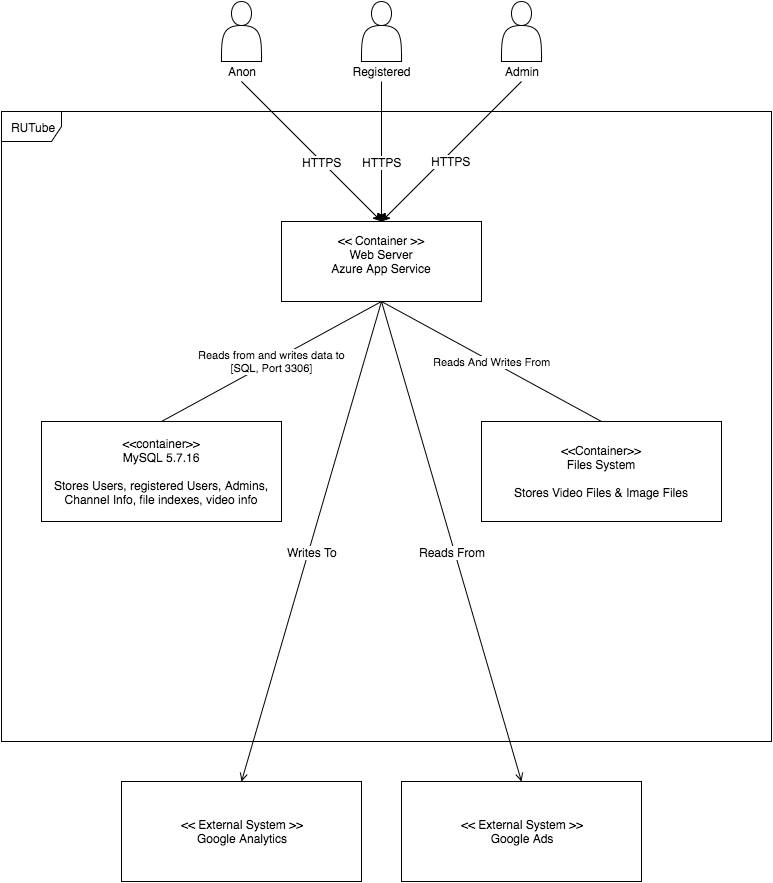
\includegraphics[height=12cm]{/Users/steinn/Documents/tolHR2016haust/T-302-HONN/Assign3honn/container_diagram.jpeg}
\newpage
	\section{Component diagram}
	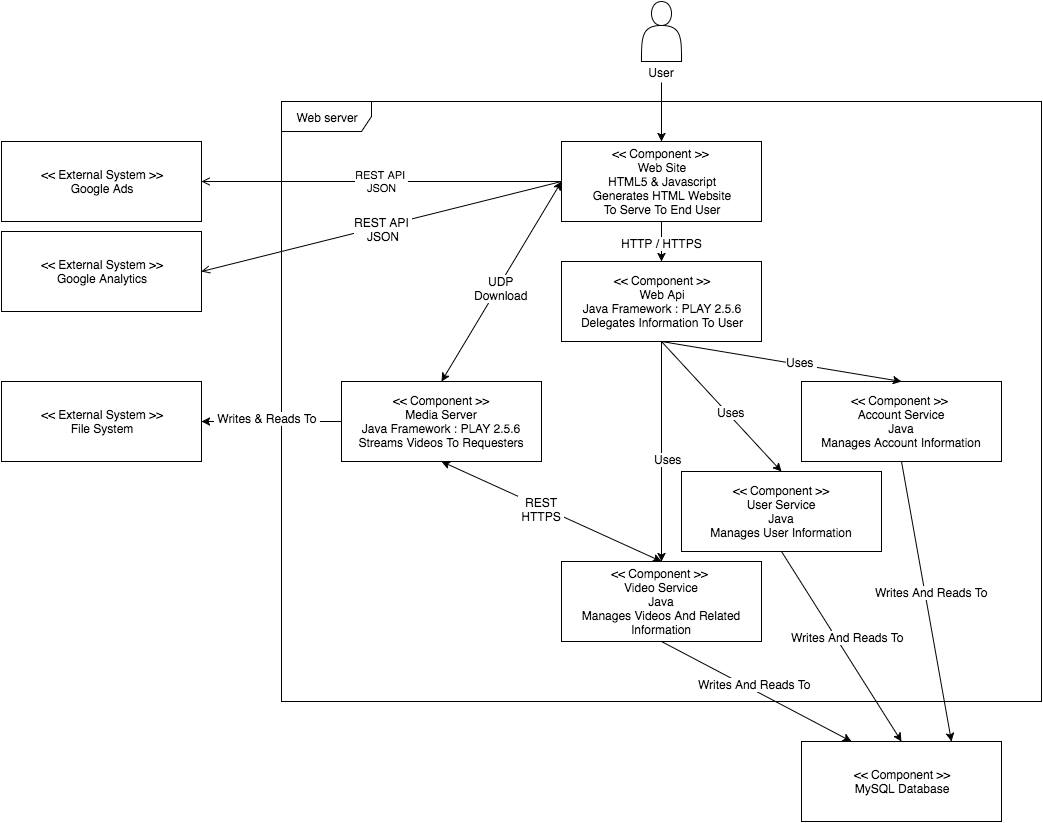
\includegraphics[height=12cm]{/Users/steinn/Documents/tolHR2016haust/T-302-HONN/Assign3honn/component_diagram.jpeg}
\newpage
	\section{REST URI}
		Following is the REST URI for the RuTube system. There are three roles in this system, anonymous user which has no authorization, regular users and admins. Above each uri call the authorization needed is specified.
		\begin{lstlisting}
For all API calls where the user needs to be logged in the
authorization header with the user token and the username header need
to be present.
Example:
{
  'Authorization': 'wegrwhrw0g9wegwe',
  'username': 'johnDoe'
}

[Authorization=none]
POST /signup
Sign up as a new user.
Example request:
  Headers:
  {
    'Content-type': 'x-www-form-url-encoded'
  }
  Body:
  {
    'fullName': 'John Doe',
    'username': 'johnDoe',
    'password': 'myPass',
    'email': 'johndoe@example.com'
  }

[Authorization=none]
POST /login
Login as an existing user with username and password
Example request:
  Headers:
  {
    'Content-type': 'x-www-form-url-encoded'
    }
  Body:
  {
    'username': 'johnDoe',
    'password': 'myPass'
  }
Example Response:
  {
    'token': '{token}',
    'username': 'johnDoe',
    'fullName': 'John Doe',
    'role': 'admin'
  }
  Where token is the session token the user sends with requests for
  authentication


[Authorization=user]
GET /profile
Displays the profile of the logged in user.
Example response:
  {
    'username': 'johnDoe',
    'fullName': 'John Doe',
    'email': 'johndoe@example.com',
    'videos': [
      {
        'id': 'funnycats',
        'title': 'Funny cats',
        'url': 'example.com/streams/funnycats',
        'creatorid': 'johnDoe'
      }
    ],
    'channels': [
      {
        'id': 'cats',
        'title': 'Cats',
        'videos': [
          {
            'id': 'funnycats',
            'title': 'Funny cats',
            'url': 'example.com/streams/funnycats',
            'creatorid': 'johnDoe'
          },
          {
            'id': 'janedoedancing',
            'title': 'Jane Doe dancing lessons part 1',
            'url': 'example.com/streams/janedoedancing',
            'creatorid': 'janeDoe'
          }
        ]
      }
    ]
  }

[Authorization=user]
PUT /profile
Modify the users settings of the logged in user.
  Example request:
  Headers:
  {
    'Content-type': 'x-www-form-url-encoded'
  }
  Body:
  {
    'fullName': 'John Doe'
  }

[Authorization=none]
GET /channels/{channelid}/videos
returns all the videos in channel with id = channelid
  Example response:
  {
    'videos': [
      {
        'id': 'funnycats',
        'title': 'Funny cats',
        'url': 'example.com/streams/funnycats',
        'creatorid': 'johnDoe'
      },
      {
        'id': 'janedoedancing',
        'title': 'Jane Doe dancing lessons part 1',
        'url': 'example.com/streams/janedoedancing',
        'creatorid': 'janeDoe'
      }
    ]
  }
  where url is the url to the streaming service

[Authorization=user]
POST /channels/{channelid}/videos
Adds a new video to channel with id = channelid
  Example request:
    Body:
    {
      'title': 'Funny cats',
      'url': 'example.com/videos?id=funnycats'
    }
  Example response:
  {
    'url': 'rutube.com/channels/cats/videos?id=funnycats'
  }
  where url is the link to the newly created video.

[Authorization=user]
POST /channels/{channelid}/subscribe
Adds the logged in user to the list of subscribers to the channel with id = channelid

[Authorization=user]
DELETE /channels/{channelid}/subscribe
Removes the logged in user from the list of subscribers to the channel with id = channelid

[Authorization=user]
DELETE /channels/{channelid}/videos?id={videoid}
Deletes a video with id = videoid from the channel with id = channelid.
To delete a video the user needs to be logged in and the one who uploaded
the video in the first place.

[Authorization=user]
GET /notifications
Checks for new videos in channels the user is subscribed to.
  Example response:
  {
    'channels': [
      {
        'id': 'cats',
        'title': 'Cats',
        'videos': [
          {
            'id': 'funnycats',
            'title': 'funny cats',
            'url': 'example.com/streams/funnycats',
            'creatorid': 'johndoe'
          },
          {
            'id': 'janedoedancing',
            'title': 'jane doe dancing lessons part 1',
            'url': 'example.com/streams/janedoedancing',
            'creatorid': 'janedoe'
          }
        ]
      }
    ]
  }

[Authorization=admin]
POST /channels
Adds a new channel to the website
  Example request:
    Body:
      {
        'title': 'Cats'
      }
  Example response:
  {
    'url': 'rutube.com/channels/cats'
  }
  where url is the link to the newly created channel.

[Authorization=admin]
DELETE /channels/{channelid}
Deletes a channel with id = channelid

[Authorization=admin]
POST /channel/{channelid}/videos/bulk
"Bulk ingests" many videos at once.
  Example request:
    Body:
    {
      'videos': [
        {
          'id': 'funnycats',
          'title': 'funny cats',
          'url': 'example.com/streams/funnycats',
          'creatorid': 'johndoe'
        },
        {
          'id': 'funnycats2',
          'title': 'funny cats 2',
          'url': 'example.com/streams/funnycats2',
          'creatorid': 'johndoe'
        }
      ]
    }

[Authorization=admin]
POST /users/bulk
"Bulk ingests many users at once"
  Example request:
    Body:
    {
      'users': [
        {
          'fullName': 'John Doe',
          'username': 'johnDoe',
          'password': 'myPass',
          'email': 'johndoe@example.com'
        },
        {
          'fullName': 'Jane Doe',
          'username': 'janeDoe',
          'password': 'myPassword',
          'email': 'janedoe@example.com'
        }
      ]
    }
		\end{lstlisting}
\newpage
	\section{Database schema}
		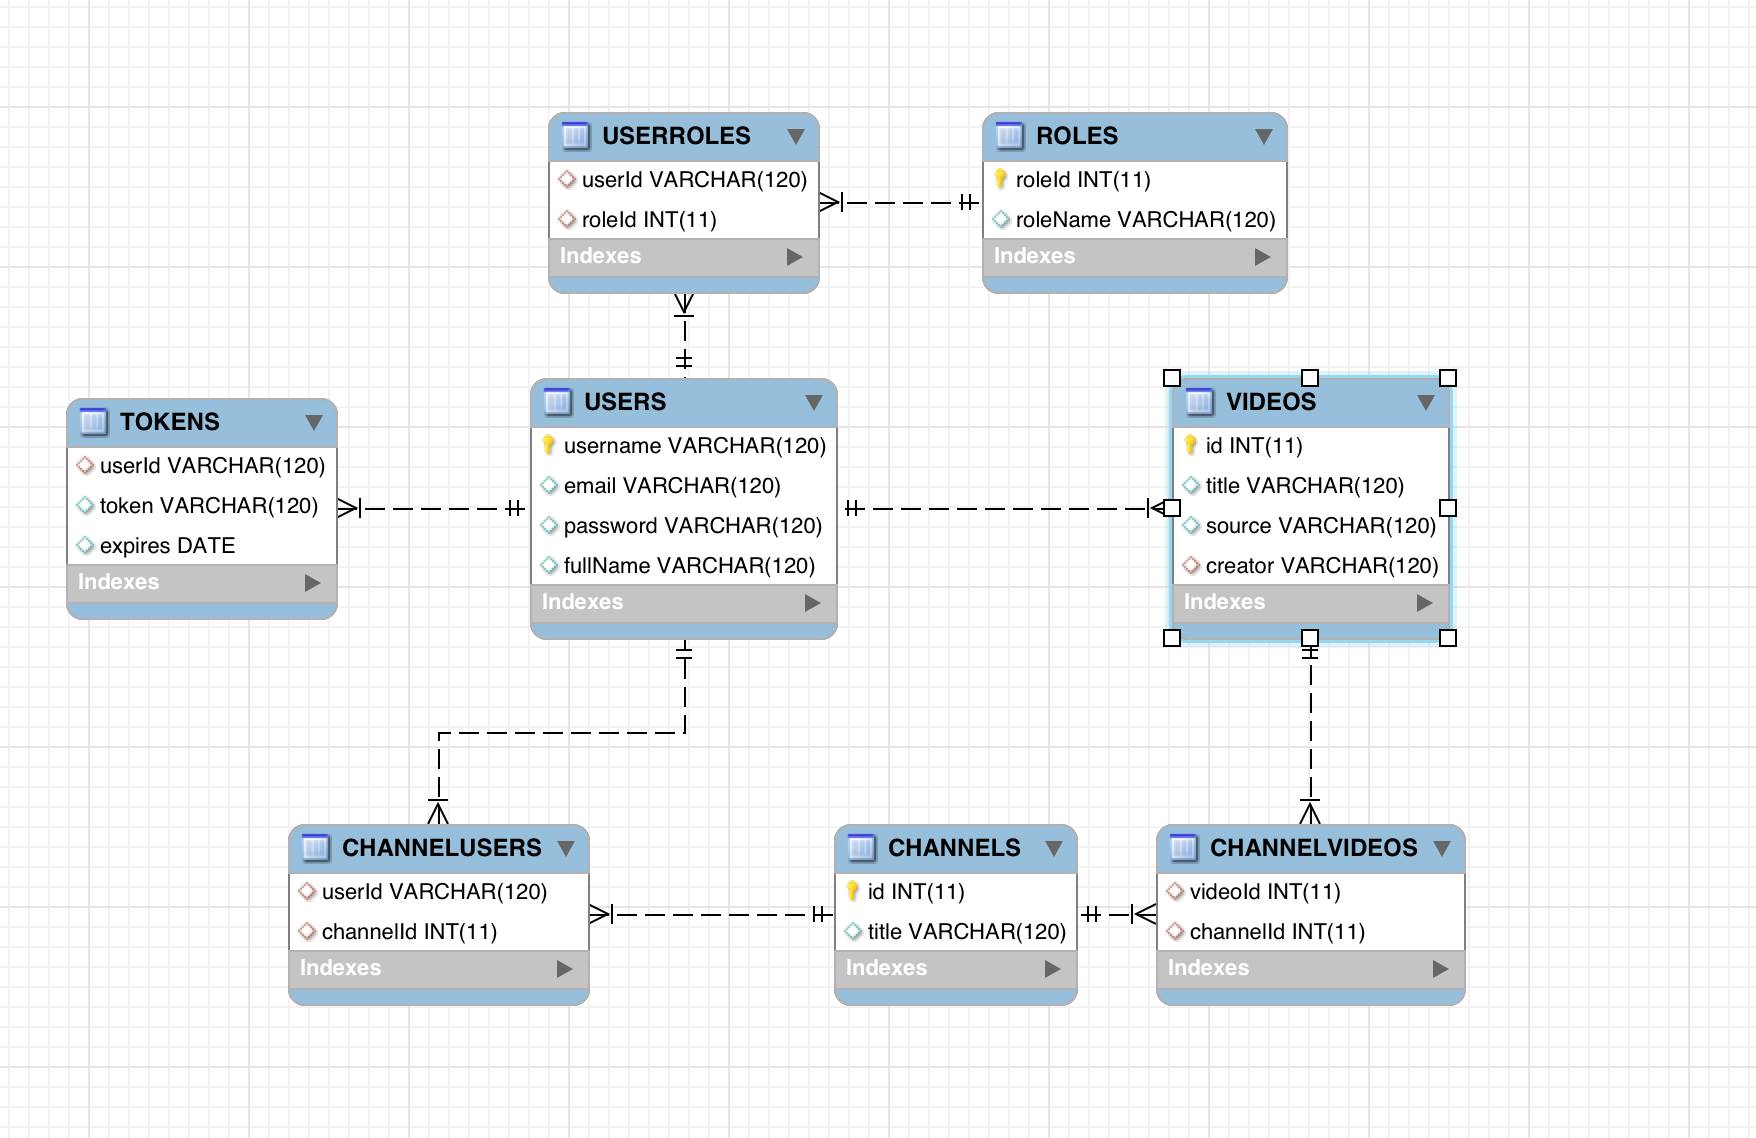
\includegraphics[height=12cm]{/Users/steinn/Documents/tolHR2016haust/T-302-HONN/Assign3honn/database_schema.jpeg}
\end{document}
